% Created 2018-04-13 Fri 15:39
% Intended LaTeX compiler: pdflatex
\documentclass[11pt]{article}
\usepackage[
top=0.75in, 
bottom=0.75in,
left=0.75in,
right=0.75in]{geometry}
\usepackage[utf8]{inputenc}
\usepackage{graphicx}
\usepackage{amsmath}
\usepackage{textcomp}
\usepackage{amssymb}
\usepackage{float}

\author{Scott Trinkle}
\date{April 16, 2018}
\title{CNR with Bandwidth}
\begin{document}

\maketitle

\section{Review of existing model}
The monoenergetic model follows the derivation in Spanne \cite{Spanne1989}:
\begin{align}
  \text{CNR}(E) = \frac{|\mu_1(E) - \mu_2(E)|}{\sqrt{\text{var}\{\mu_1(E)\} + \text{var}\{\mu_2(E)\}}},
  \label{eq:CNR}
\end{align}
where $\mu_1(E) \equiv \mu_{bg}(E)$ is the attenuation at the center voxel of a
homogeneous spherical object of material ``bg'' and
$\mu_2(E) \equiv \mu_{bg}(E) + \mu_c(E)$ is the attenuation of that same voxel
with the addition of a small amount of contrast material ``c.'' (In these notes,
$i \in [1,2]$ will index these two cases).

The variance is defined as
\begin{align}
  \text{var}\{\mu_i(E)\} \propto \frac{1}{\bar{N}_i(E)},
  \label{eq:var}
\end{align}
where
\begin{align}
  \bar{N}_i(E) &= I_0(E) \text{ exp}\left\{-A_i(E)\right\}.
\end{align}
Here, $I_0(E)$ is the incident intensity (assumed monoenergetic for now), and
$A_i$ is given by
\begin{align}
  A_i(E) = \sum_{j}\mu_j(E) d_j,
  \label{eq:Ai}
\end{align}
where $d_j$ is the length of each material, $j$, that is present in case $i$.

\section{Bandwidth}

We would like to introduce the spectral bandwidth, $BW$, into this model. We
define $BW$ as follows:
\begin{align}
  BW = \frac{\Delta E}{E} = 10^{-2}\text{ or } 10^{-4},
\end{align}
where $\Delta E$ is the FWHM of the intensity function $I_0(E)$.
We model the intensity function as:
\begin{align}
  I_0(E) = I_0 N(E | E, \sigma_{E,BW}),
\end{align}
where $I_0$ is a constant intensity and $N$ is a normalized Gaussian function with mean
$E$ and standard deviation $\sigma_{E, BW}$:
\begin{align}
  \sigma_{E,BW} = \frac{E\cdot BW}{2\sqrt{2\text{ln}2}},
  \label{eq:sigma}
\end{align}
calculated from the FWHM of the spectrum at energy $E$.

We can incorporate this expression into our model for $\bar{N}_i(E)$ as
\begin{align}
  \bar{N}_i(E) = I_0\int_0^{\infty} dE'N(E' | E, \sigma_{E,BW})\text{ exp}\{-A_i(E')\},
  \label{eq:Ni}
\end{align}
and the variance and CNR are calculated as before.

\section{Implementation}
The mass attenuation data for ``bg'' (water) and ``c'' (Os, U or Pb) materials
is taken from the NIST database. The sampled energy points for these databases
are generally nonuniform and different for each material, with some materials
requiring finer sampling around sharp absorption peaks. Accordingly, after the
two materials are chosen, the attenuation data for the less densely sampled
material is logarithmically interpolated onto the sampled energy points of the
more densely sampled material, so they share the same array of E values from
$\sim$0-100 keV.

The integral in Eqn.~\ref{eq:Ni} is then implemented with the following logic:\newline

For each energy value $E_k$ in the common energy array $E_{arr}$,
\begin{itemize}
\item Calculate $\sigma_{E_k,BW}$ according to Eqn~\ref{eq:sigma}
\item Define an $n$-length $E'$ array: $E' \in [E_k-r\sigma_{E_k, BW}, E_k+r\sigma_{E_k, BW}]$
  \begin{itemize}
  \item $r$ defines the truncation width 
  \item Replace conflicting boundary values in $E'$ with min($E_{arr}$) or max($E_{arr}$) as needed
  \end{itemize}
\item Calculate the $n$-length array $A_i(E')$ with Eqn.~\ref{eq:Ai} using
  $\mu_i(E')$ logarithmically interpolated once more from the NIST data
\item Calculate $N$, the $n$-length array of normalized Gaussian weights for $E'$
  \begin{itemize}
  \item With mean $E_k$ and standard deviation $\sigma_{E_k,BW}$
  \end{itemize}
\item $\bar{N}_i(E_k)$ is then calculated as
  \begin{align}
    \bar{N}_i(E_k) = \text{sum}(N\cdot\text{exp}\{-A_i(E')\}),
  \end{align}
  where $\cdot$ indicates an element-wise product.
  
\end{itemize}

The CNR is then calculated as before, with Eqns~\ref{eq:CNR} and~\ref{eq:var}. I
have been using $n=50$ and $r=4$. Many of these arrays can be pre-computed,
which speeds up the actual implementation.

A sample implementation is shown in Figure~\ref{fig:results} for $BW=0$
(monoenergetic), $BW=10^{-2}$ and \newline$BW=10^{-4}$. The inset shows detail
near the finest structure of the monoenergetic plot, and the bottom plot
shows the absolute percent difference as a function of energy. 

\begin{figure}[H]
  \centering
  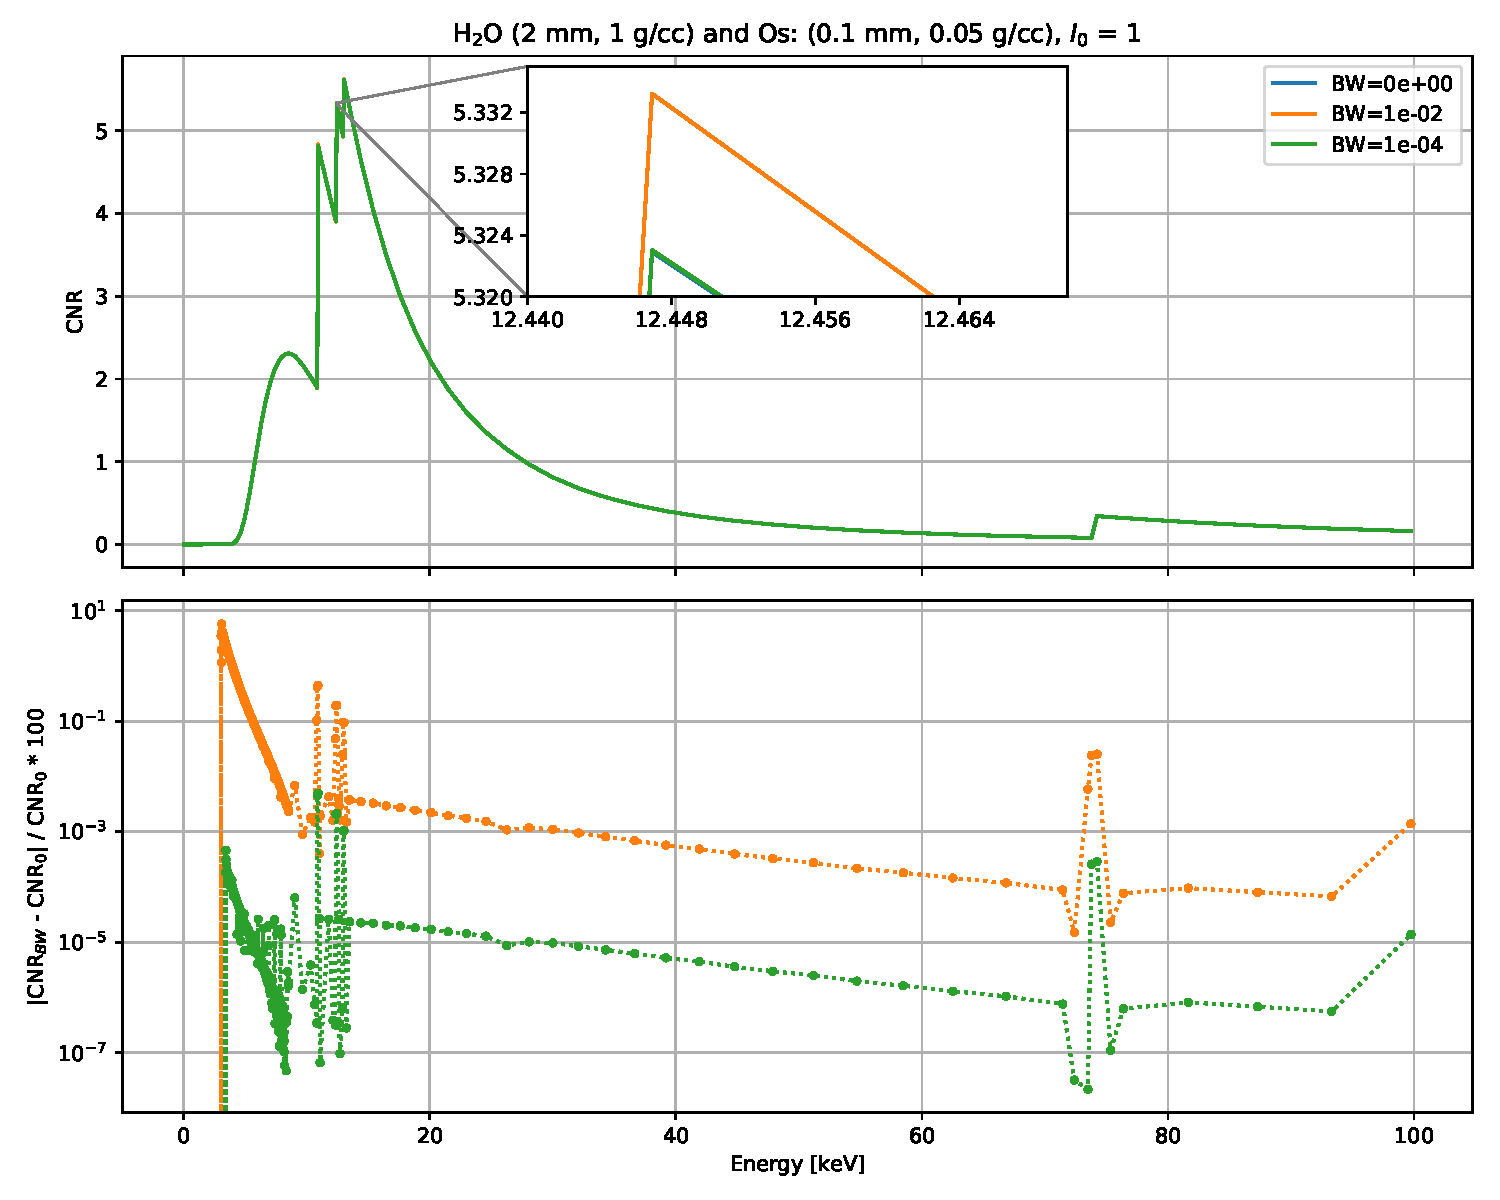
\includegraphics[width=\linewidth]{cnrwithbw}
  \caption{Results for CNR with bandwidth.}
  \label{fig:results}
\end{figure}

\bibliographystyle{ieeetr}
\bibliography{report}
\end{document}